\documentclass[../main.tex]{subfiles}

\begin{document}

\chapter{Trabalhos Relacionados}\label{cap:relacionados}

Os trabalhos relacionados a este podem ser amplamente classificados em ferramentas de autoria tradicionais para apresentações multimídia, ferramentas de autoria baseadas em RA, e interfaces de usuário tangíveis. Cada uma dessas categorias são discutidas nas Seções \ref{sec:ferramentas_multimidia}, \ref{sec:ferramentas_ra}, e \ref{sec:interfaces_tangiveis}.

\section{Ferramentas de autoria para apresentações multimídia}
\label{sec:ferramentas_multimidia}

De modo similar a ferramentas de autoria para apresentações multimídia--- como GRiNS~\cite{bulterman_grins_1998}, %
LimSee3~\cite{deltour_limsee3_2006}, %
Adobe Animate~\cite{adobe_animate_2017}, %
NEXT~\cite{paulo_de_mattos_next_2013}, %
e NCL~Composer~\cite{azevedo_composer_2014}%
--- o principal objetivo deste trabalho é permitir que usuários sem habilidades com programação criem conteúdo multimídia.

A ferramenta GRiNS~\cite{bulterman_grins_1998} é um ambiente de autoria e apresentação que pode ser usado para criar e tocar documentos SMIL\cite{rutledge2001smil} criados com a própria ferramenta ou fora dela. SMIL é uma linguagem declarativa para a descrição de documentos multimídia baseados em Web. A Figura \ref{fig:grins} mostra conteúdo multimídidia criado utilizando a ferramenta GRiNS em que ocorre o aumento de informação durante a transmissão de um jornal, em que informações adicionais sobre o âncora são mostradas. Diferente dessa ferramenta, que é baseada no paradigma da linguagem SMIL, a abordagem proposta é baseada no modelo do contexto aninhado, do inglês \emph{Nested Context Model}~(NCM)\cite{soares_nested_2005}.

\begin{figure}[!h]
\centering
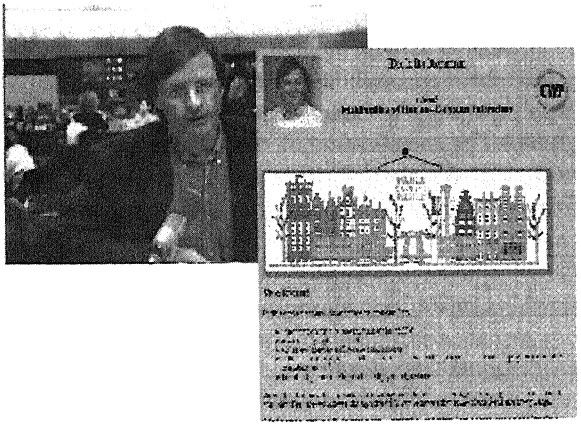
\includegraphics[width=0.5\linewidth]{IMG/Relacionados/grins.png}
\caption{Aumentando informação durante um jornal.}
\fonte{\citeonline{bulterman_grins_1998}}
\label{fig:grins}
\end{figure}

LimSee3~\cite{quint_nouguier_2019} é uma ferramenta de autoria baseado no modelo homônimo~\cite{deltour_limsee3_2006}. Tal modelo utiliza \emph{templates} enquanto mantém ricas capacidades de composição. LimSee3 é uma evolução da ferramenta LimSee2~\cite{deltour2005limsee2}~(uma ferramenta de autoria para a linguagem SMIL). A Figura \ref{fig:limsee3} mostra a interface da ferramenta LimSee3. Como mencionado anteriormente, a abordagem proposta neste trabalho é baseada no modelo NCM, diferente da ferramenta LimSee3.

\begin{figure}[!h]
\centering
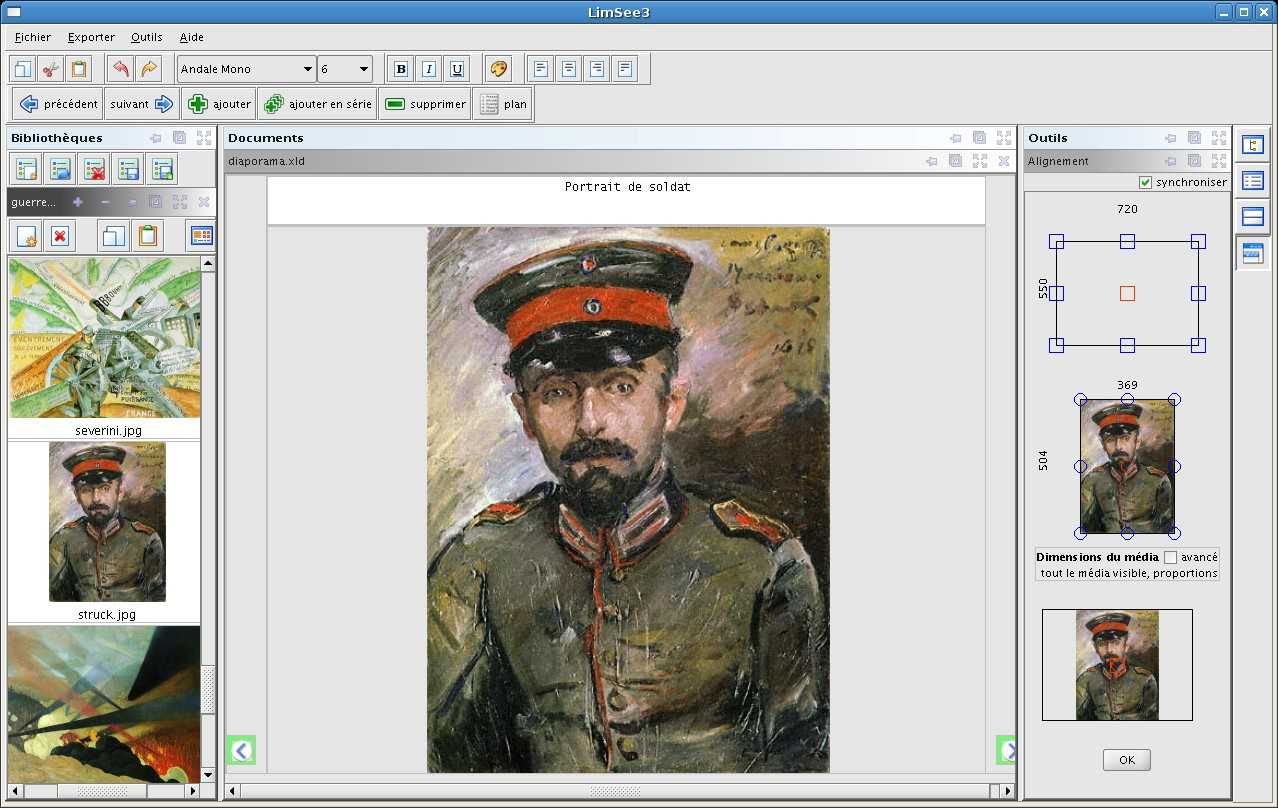
\includegraphics[width=0.5\linewidth]{IMG/Relacionados/limsee3.jpg}
\caption{Interface da ferramenta LimSee3.}
\fonte{Site do projeto LimSee3 \cite{quint_nouguier_2019}}
\label{fig:limsee3}
\end{figure}


A ferramenta Adobe Animate \cite{adobe_animate_2017} é uma ferramenta proprietária de autoria multimída e animação computacional. Tal ferramenta é utilizada para a criação de conteúdo para o Adobe Flash Player~\cite{adobe_flash2019}, tais como aplicações para a internet, jogos e desenhos animados. A Figura \ref{fig:adobe} mostra a interface da ferramenta Adobe Animate. Por ser uma ferramenta proprietária, maiores informações sobre o modelo em que a ferramenta é baseada não estão disponíveis.

\begin{figure}[!h]
\centering
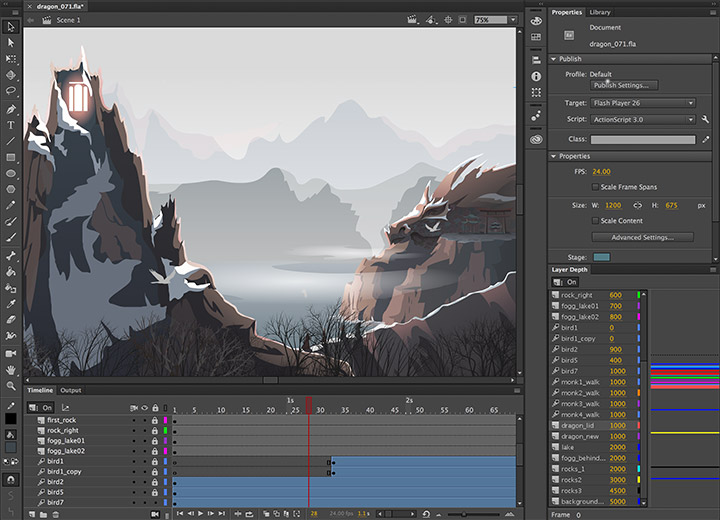
\includegraphics[width=0.5\linewidth]{IMG/Relacionados/adobe.jpg}
\caption{Interface da ferramenta Adobe Animate.}
\fonte{Site da ferramenta Adobe Animate~\cite{adobe_animate_2017}}
\label{fig:adobe}
\end{figure}


Diferente dessas ferramentas, a abordagem proposta não utiliza o modo tradicional de interface (baseada em janelas, ícones e menus), mas explora o uso de RA e objetos do mundo real (marcadores) para especificar o comportamento e relações entre \emph{objetos de mídia} na apresentação. Desta feita, este trabalho explora uma nova metáfora para a autoria de conteúdo multimídia, que pode também estimular e entreter o usuário simultaneamente.

Em particular, apesar de usar uma técnica de interação diferente, o modelo conceitual da proposta BumbAR é baseado no modelo NCM~(Nested Context Model)~\cite{soares_nested_2005}, que também é sedo pela abordagem baseada em interface gráfica comum da NCL Composer~\cite{azevedo_composer_2014}. A ferramenta BumbAR também exporta o conteúdo criado para NCL (Nested Context Language)~\cite{soares_programando_2009}, permitindo que a apresentação criada seja tocada em aparelhos de TV digital ou navegadores web (usando WebNCL~\cite{melo_webncl_2012} ou NCL4Web~\cite{silva_ncl4web_2013}, por exemplo).

\section{Ferramentas de autoria baseadas em RA}
\label{sec:ferramentas_ra}

Apesar da maioria do conteúdo em RA ainda ser criado por desenvolvedores de sistemas, algumas ferramentas de autoria foram propostas para criar conteúdo em realidade aumentada. Elas geralmente fornecem ferramentas complexas para designers modelarem objetos tridimensionais e associá-los com objetos físicos e marcadores. A maioria delas, entretanto, ainda segue um abordagem baseada em uma interface gráfica com o usuário, do inglês \emph{graphical user interface(GUI)}. Exemplos dessa abordagem são as seguintes ferramentas: MARS Authoring Tool~\cite{sinem_authoring_2003}, DART~\cite{macintyre_dart_2004}, ComposAR~\cite{seichter_composar_2008}, AuthorAR~\cite{lucrecia_authorar_2013}, Lagarto~\cite{maia_lagarto_2017}. Outras ferramentas, mais relacionadas a este trabalho, proporcionam uma abordagem imersiva ou mista (interface gráfica comum em conjunto com um ambiente imersivo) para a criação de conteúdo RA.

Por exemplo, \citeonline{langlotz_sketching_2012} apresenta um sistema para criar conteúdo RA baseados em dispositivos móveis. Tal sistema possui como público alvo uma audiência inexperiente. Através da interação direta com o dispositivo móvel usando a tela sensível ao toque, o sistema permite que autores criem e registrem primitivas 3D, modificar primitivas 3D registradas, aplicar textura aos objetos 3D registrados e gerem objetos 2D registrados~(que podem servir como anotações). Embora a proposta seja interessante, não há uma avaliação com o público alvo da proposta. Assim, é difícil saber quão bom o sistema é na visão dos usuários finais.

Os trabalhos de \citeonline{vera_situar_2016} e \citeonline{sucar_platform_2017} também apresentam um trabalho em andamento no desenvolvimento de uma ferramenta de autoria baseada em RA, chamada de SituAR, para criar conteúdo RA \emph{in-situ}. O principal objetivo da proposta é aumentar, no sentido de realidade aumentada, pontos de interesse, do inglês \emph{points of interest~(POIs)} para cidades inteligentes. Como características previstas para o SituAR, os autores mencionam: criar e visualizar anotações, visualização de mapa, e expandir anotações próximas. Como mencionado, a abordagem proposta ainda é um projeto em andamento, e os trabalhos citados não fornecem detalhes suficientes para uma comparação mais detalhada.

Diferente das ferramentas de autoria para a criação de conteúdo RA mencionadas acima, o conteúdo criado pela proposta deste trabalho não é conteúdo RA. O principal objetivo é explorar RA como uma forma inovadora de interface com o usuário para criação de apresentações multimídia tradicionais~(composta de imagens, vídeos, músicas, etc.).

De maneira similar à proposta deste trabalho, \citeonline{shin_ar_2005} também possuem o objetivo de criar um ferramenta de autoria baseada em RA para criar conteúdo não aumentado. A ferramenta baseada em RA posposta por \citeonline{shin_ar_2005} tem o intuito de criar \emph{storyboards}(série de imagens ou desenhos que mostram a evolução de uma animação ou vídeo). Com o uso do \emph{item block}(marcador RA) proposto no trabalho, é possível a especificação de personagens, informação de plano de fundo, propriedades de palco, ações, e expressões faciais. Através do posicionamento de itens baseados em personagens na visão da câmera, é possível determinar a pose dos modelos tridimensionais correspondentes na cena. Componentes dinâmicos, como ações e expressões faciais, podem ser posicionadas em qualquer lugar dentro do campo de visão da câmera. Apesar de possuírem natureza diferente~(o presente trabalho está interessado principalmente no comportamento temporal de uma apresentação multimídia enquanto \citeonline{shin_ar_2005} estão interessados em \emph{storyboards} para cenas tridimensionais) a fase de criação de elos (detalhada na Seção \ref{subsec:criacao_elos}) proposta neste trabalho tem relação com os componentes dinâmicos propostos por \citeonline{shin_ar_2005}. Entretanto, um dos pontos negativos do trabalho mencionado é a não realização de uma avaliação com possíveis usuários.

Finalmente, apesar deste trabalho estar especialmente interessado na especificação do comportamento de apresentações multimídia tradicionais, alguns conceitos e técnicas de interação apresentadas neste trabalho podem também ser úteis para outras ferramentas de autoria baseadas em RA (para a criação de conteúdo RA ou tradicional). Em especial, os conceitos de eventos do modelo NCM, no qual este trabalho é baseado, podem ser úteis para a especificação do comportamento de conteúdo RA. Entretanto, uma investigação dessa possibilidade está além do escopo deste trabalho, e é deixada como um possível trabalho futuro. 

\section{Interfaces de usuário tangíveis}
\label{sec:interfaces_tangiveis}

Outra área relacionada a este trabalho é a de interfaces de usuário tangíveis~\cite{ishii_tangible_2008}. O principal objetivo dessa área é propiciar interfaces tangíveis para que usuários possam usar objetos físicos tradicionais como elemento interativos com o computador. De fato, tecnologias RA podem ser usadas como uma base para facilitar o desenvolvimento de diversas interfaces tangíveis, e existem diversos exemplo integrando-os. 

Por exemplo, \citeonline{ha_artalet_2010} propõe uma abordagem que mistura elementos de uma interface gráfica, do inglês \emph{graphical user interface}(GUI) com uma interface tangível, do inglês \emph{tangible user interface}(TUI) para criar conteúdo RA. No trablago, os autores propõem uma ferramenta de autoria para livros eletrônicos, do inglês \emph{eBook}, aprimorados com elementos RA. A interface tangível é composta de uma caixa cúbica acoplável a um mouse e com múltiplos marcadores impressos na caixa. De modo similar, como ficará mais claro no restante deste trabalho, a presente proposta também provê uma interface tangível (baseada em marcadores RA) em que os autores criam conteúdo através da interação com objetos físicos. Entretanto, diferentemente, o principal foco é em uma interface para a criação de apresentações multimídia.

\end{document}